\documentclass[12pt,a4paper]{article}
\usepackage[utf8]{inputenc} %codificacao de entrada
\usepackage[T1]{fontenc} %codificacao de saida
\usepackage[brazil]{babel}

\usepackage{titling}		% arruma pre titulo
\usepackage{makeidx}        % Cria o indice
\usepackage{hyperref}       % Controla a formacao do indice
\usepackage{lastpage}       % Usado pela Ficha catalografica
\usepackage{indentfirst}    % Indenta o primeiro paragrafo de cada secao.
\usepackage{xcolor}          % Controle das cores
\usepackage{graphicx}       % Inclusao de graficos
\usepackage{placeins}
\usepackage{subfig}
\usepackage{amsmath}        % pacote matemático
\usepackage{listings}
\usepackage{longtable}
\usepackage{float}

\usepackage[hmargin=2cm,vmargin=3.5cm,bmargin=2cm]{geometry}

\pretitle{%
  \begin{center}
  \LARGE
  
\includegraphics[width=3.5cm,height=4cm]{imgs/logo.png}\\[1.5cm]\textbf{Universidade do Estado do Rio de Janeiro}\\ Instituto Politécnico\\Engenharia de Computação\\[2cm]
}
\posttitle{\normalsize \end{center}}

\title{\textbf{\underline{Trabalho}\\[0.5cm]
Processos Estocásticos}\\[0.3cm]\large{Professor Angelo}\\[1.5cm]}
\author{
	Ana Carolina Castro\\
	\texttt{anacarolinacastro@aol.com}
	\and
	Ciro Chang\\
	\texttt{cirochang@live.com}
	\\[1.5cm]
}
\date{Nova Friburgo\\31 de Outubro de 2015}

    
\begin{document}
\maketitle
\thispagestyle{empty}

\newpage
\tableofcontents

\newpage
\section{Introdução}
Esse trabalho tem como objetivo 

\newpage
\section{O Passeio Aleatório}
O Passeio Aleatório, ou Caminhante Bêbado, é um modelo aonde um caminhante dá um passo em uma direção aleatória. Podemos tomar como exemplo o caminho percorrido por uma molécula ou por um fluido. O algoritmo do Passeio Aleatório é dado pelas seguintes regras" o caminhante tem um ponto de partida inicial, ele anda um passo constante em uma direção, a direção é escolhida aleatoriamente e todas as direções tem a mesma probabilidade de escolha.



\subsection{Desvio padrão}
Na área da Probabilidade e Estatística, o desvio padrão é a medida mais comum da dispersão estatística. Sua principal característica é mostrar o quanto de variação existe em relação a média esperada. A fórmula utilizada para calcular o desvio padrão das simulações realizadas foi a equação \ref{desvio}.

\begin{equation}
\label{desvio}
s = \sqrt{\frac{\sum{x_i^2} - \frac{1}{n}(\sum{x_i)^2}}{n}}
\end{equation}

\subsection{O Caminhante em uma dimensão}
Quando admitimos que o caminhante passeia em apenas uma dimensão, consideramos que ele anda em $y$, podendo ir para cima ou para baixo. Como na figura \ref{um_caminhante1}.

\begin{figure}[H]
\centering
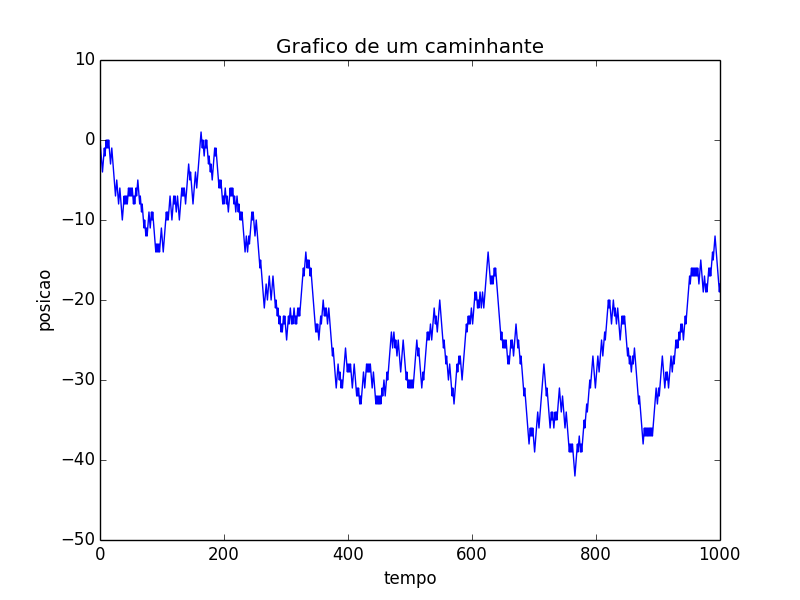
\includegraphics[width=12cm,height=9cm]{imgs/1d/um_caminhante.png}
\caption{Caminho percorrido por apenas um caminhante em uma dimensão}
\label{um_caminhante1}
\end{figure}


Usamos essa simulação para calcular o caminho de 1000 passos, percorrido por 1000 caminhantes. Como resultado obtivemos o seguinte histograma (figura \ref{histograma1}).

\begin{figure}[H]
\centering
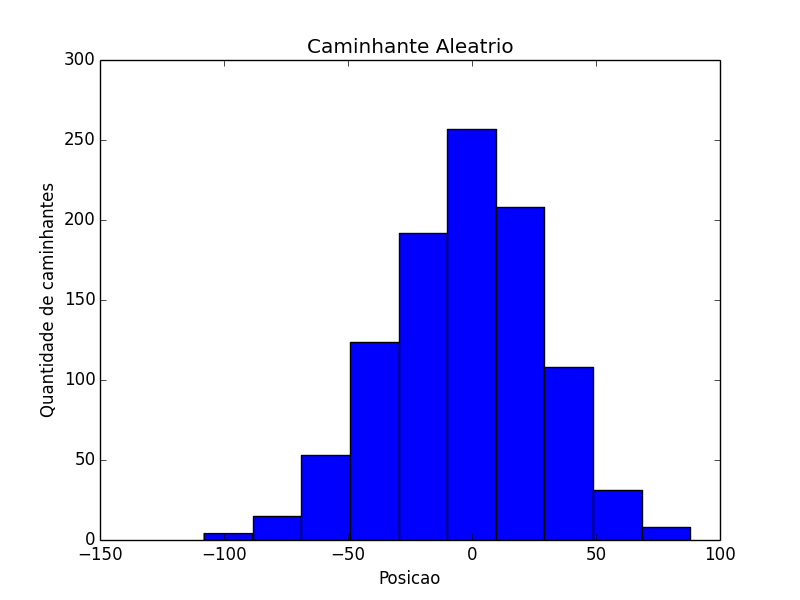
\includegraphics[width=12cm,height=9cm]{imgs/1d/histograma.png}
\caption{MUDAR A LEGENDA}
\label{histograma1}
\end{figure}

Calculamos o desvio padrão para as amostras calculadas dos caminhantes (figura \ref{desvio1}).

\begin{figure}[H]
\centering
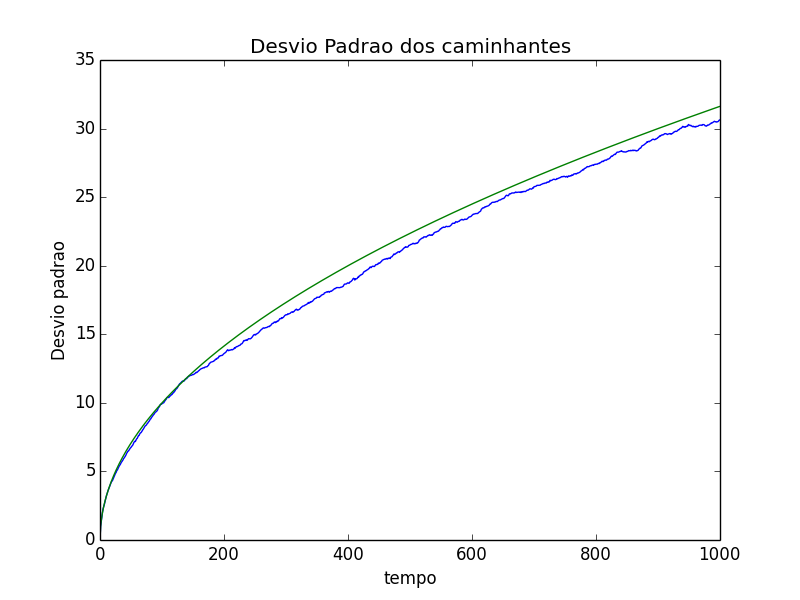
\includegraphics[width=12cm,height=9cm]{imgs/1d/desvio.png}
\caption{MUDAR A LEGENDA}
\label{desvio1}
\end{figure}

\newpage
\subsection{O Caminhante em duas dimensões}
Quando admitimos que o caminhante passeia em duas dimensões, consideramos que ele anda em $x$ ou $y$, podendo andar em $x$ e $y$ ao mesmo tempo ou só em $x$ ou $y$ (cima, baixo, esquerda, direita e diagonais).Como na figura \ref{um_caminhante2}.

\begin{figure}[H]
\centering
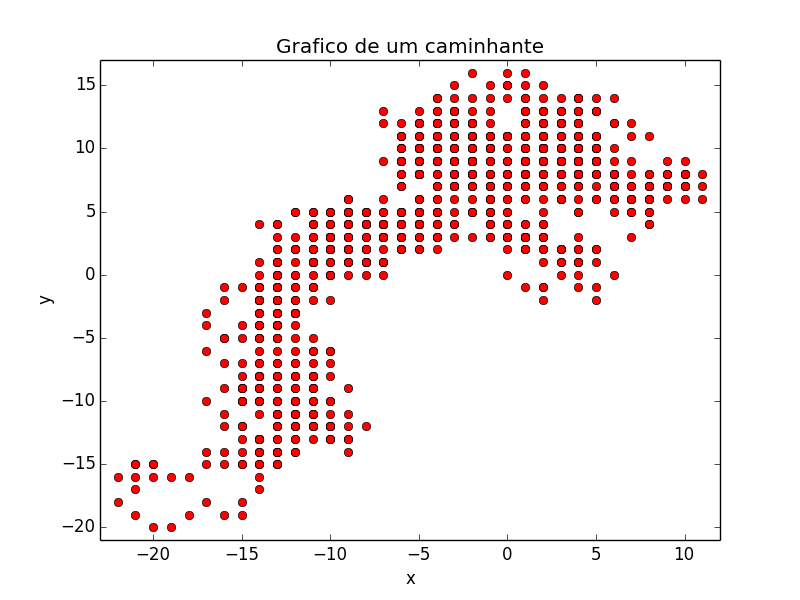
\includegraphics[width=12cm,height=9cm]{imgs/2d/um_caminhante.png}
\caption{Caminho percorrido por apenas um caminhante em uma dimensão}
\label{um_caminhante2}
\end{figure}

Usamos essa simulação para calcular o caminho de 1000 passos, percorrido por 1000 caminhantes. Como resultado obtivemos o seguintes histogramas para o eixo $x$ (figura \ref{histograma2x}) e para o eixo $y$ (figura \ref{histograma2y}).

\begin{figure}[H]
\centering
\includegraphics[width=12cm,height=9cm]{imgs/2d/histograma_X.png}
\caption{MUDAR A LEGENDA}
\label{histograma2x}
\end{figure}

\begin{figure}[H]
\centering
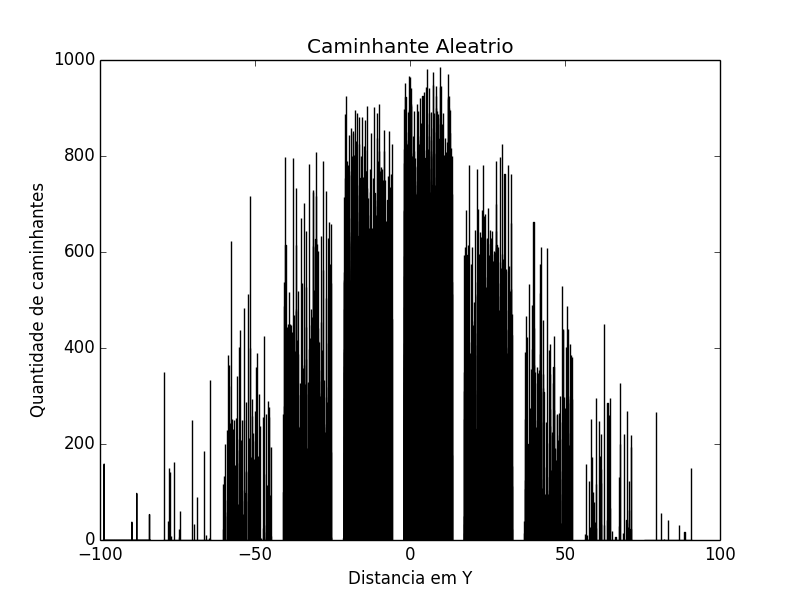
\includegraphics[width=12cm,height=9cm]{imgs/2d/histograma_y.png}
\caption{MUDAR A LEGENDA}
\label{histograma2y}
\end{figure}


Calculamos o desvio padrão para as amostras calculadas dos caminhantes (figura \ref{desvio2}). O desvio padrão para o caminhante 2D foi calculado com base nos desvios em relação a X e a Y e calculamos a norma desses dois resultados.


\begin{figure}[H]
\centering
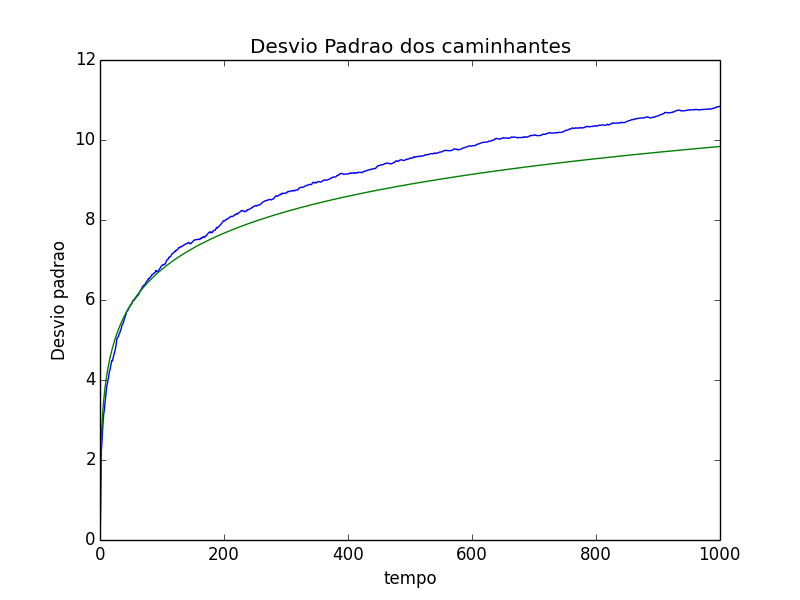
\includegraphics[width=12cm,height=9cm]{imgs/2d/desvio.png}
\caption{MUDAR A LEGENDA}
\label{desvio2}
\end{figure}


\newpage
\section{Experimento da Gota}
O propósito dessa seção é comparar a simulação do Passeio Aleatório e o Experimento da Gota.

\subsection{O Experimento}
No experimento, foi analisado a dispersão de um traçador (tinta de caneta permanente) em uma superfície de papel. Filmamos a movimentação das moléculas da tinta no papel e separamos em 18 frames (figura \ref{frames}). Utilizando a biblioteca 'PIL' (Python Image Library), calculamos quantos pixels de cada frame eram pretos, ou cores próximas ao preto. A partir da contagem dos pixels, calculamos o raio da gota (no tempo $t$) utilizando a fórmula (\ref{area}) da área de uma circunferência. Desse modo, passamos a ter os raios da gota para cada um dos tempos (frames).

\begin{figure}[H]
\centering
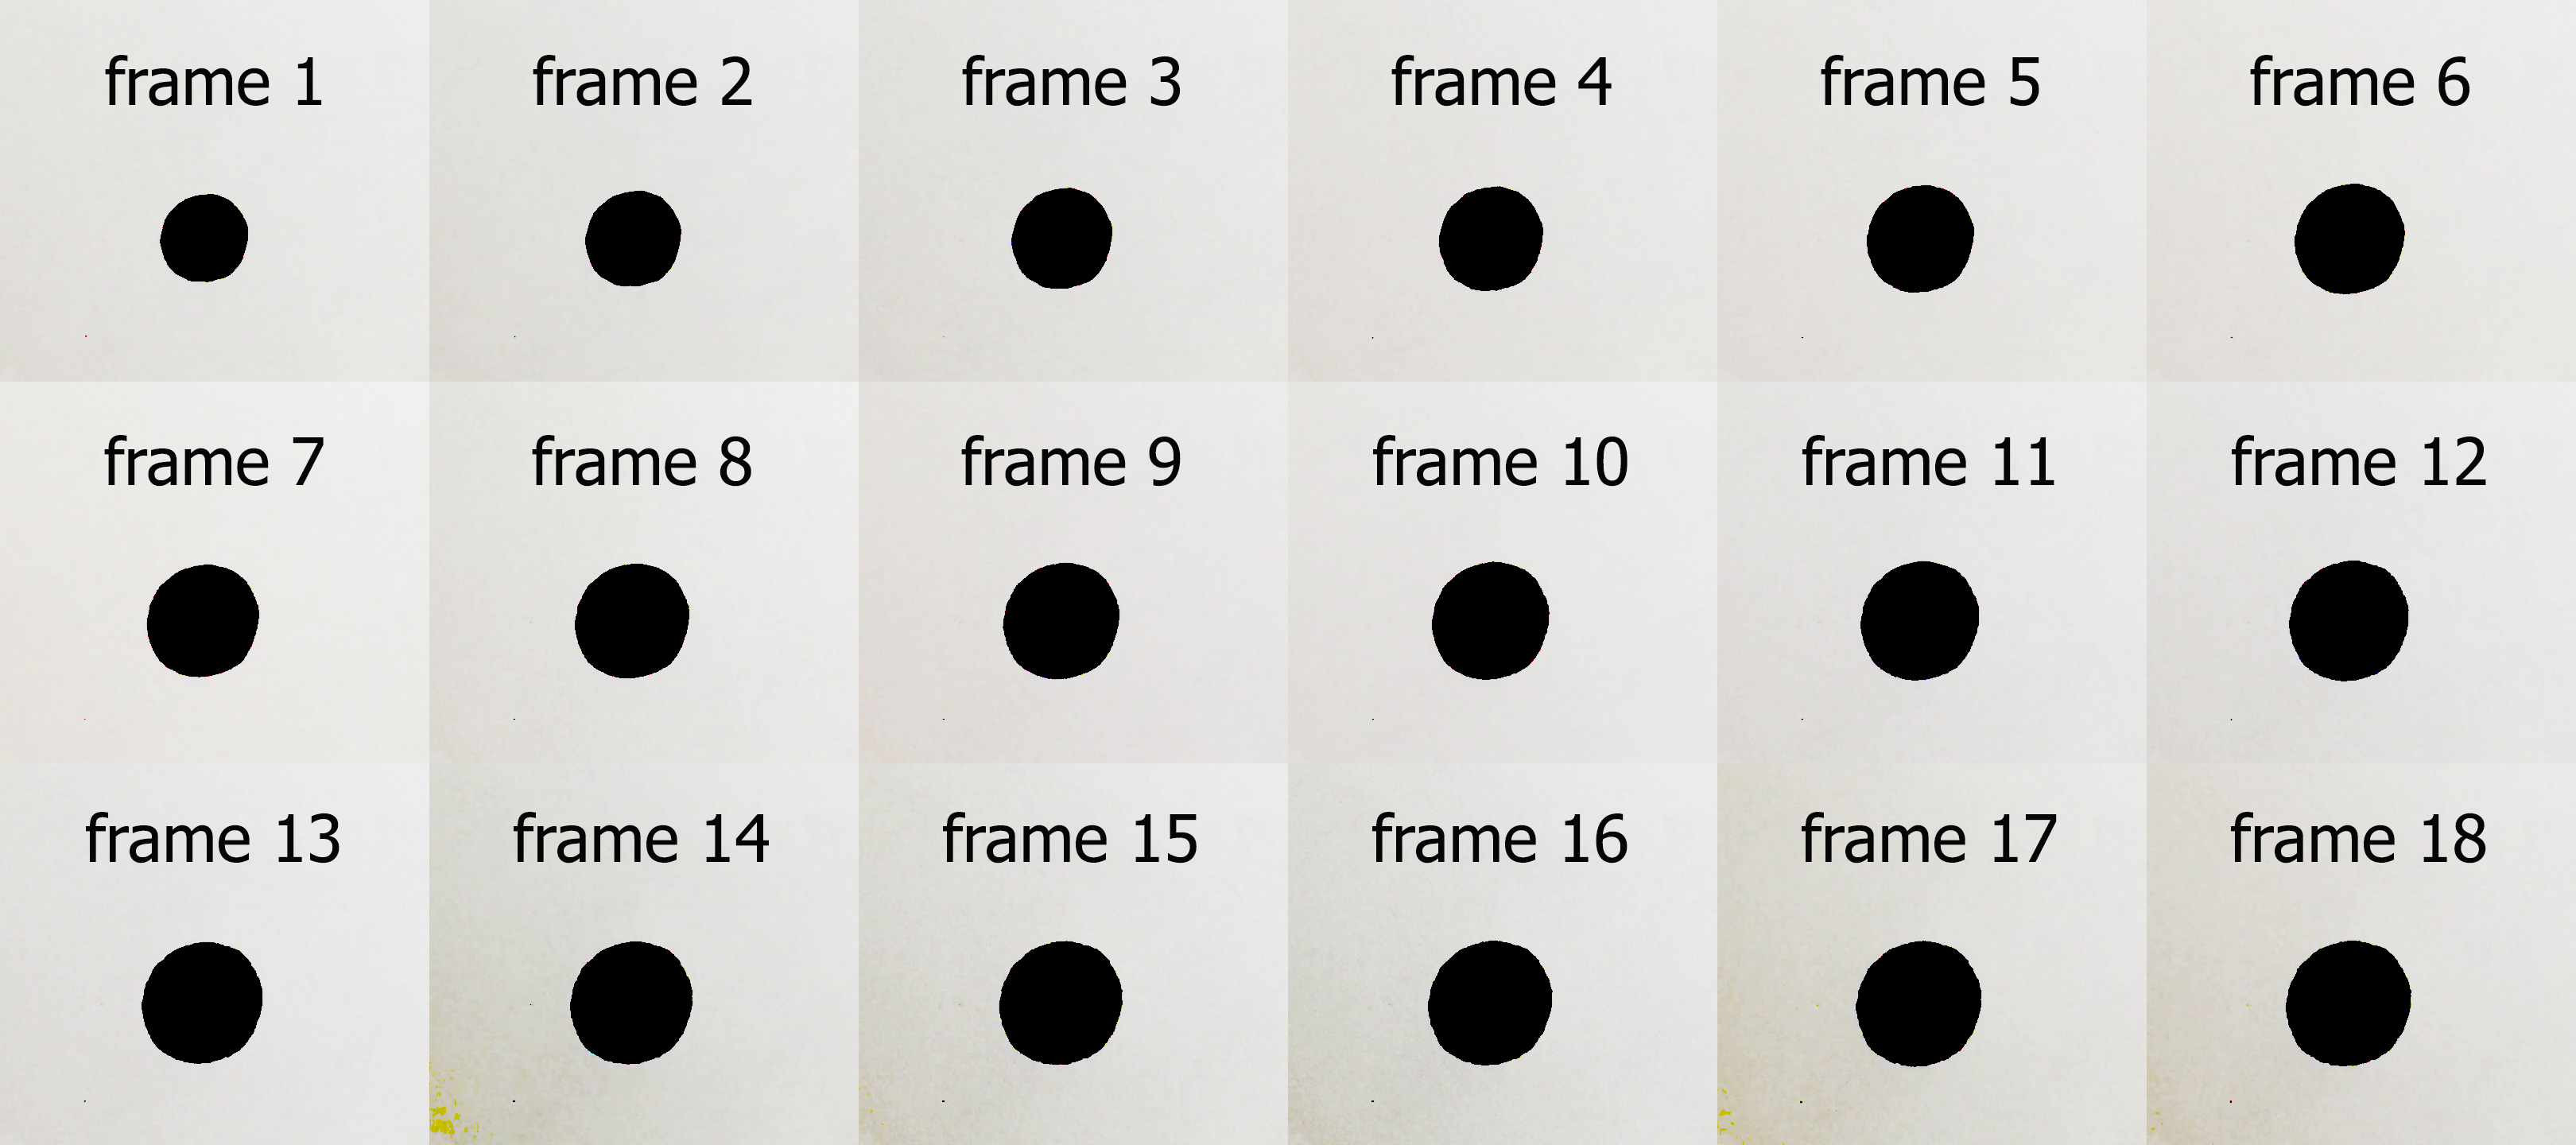
\includegraphics[width=13cm,height=6cm]{imgs/frames.jpg}
\caption{Frames da gota dispersando.}
\label{frames}
\end{figure}

\begin{subequations}
 \label{area}
 \begin{align}
A =  \pi r^2\\
r = \sqrt{\frac{A}{\pi}}
 \end{align}
\end{subequations}

\newpage
\subsection{Resultados}
A partir dos frames, conforme explicado na subseção anterior, obtivemos os seguintes (tabela \ref{raios}) valores para o raio da gota no determinado instante.

\begin{table}[H]
\centering
\caption{Valores dos raios.}
\label{raios}
\begin{tabular}{|c|c|}
\hline
\textbf{frame} & \textbf{r}  \\
\hline
1          & 0.0000000000000000    \\
2          & 4.8614531096986300    \\
3          & 7.9622103949172285    \\
4          & 10.318877638434742    \\
5          & 12.279599156048462    \\
6          & 14.004704563355219    \\
7          & 15.301347744326350    \\
8          & 16.881628115741066    \\
9          & 17.742845371250354    \\
10        & 18.157515625751387    \\
11        & 19.149235447234418    \\
12        & 19.943364081042446    \\
13        & 20.673835708371385    \\
14        & 21.485613609689835    \\
15        & 22.109636622936847    \\
16        & 22.658230422829476    \\
17        & 23.135058014571882    \\
18        & 23.138279661173150  \\
\hline  
\end{tabular}
\end{table}

Ao observar esses resultados, podemos notar que gota tende a ficar com o raio próximo à $23.14$ pixels.

Fitamos esses valores a fim de verificar se o gráfico se aproxima do gráfico $\sqrt{t}$, assim como no modelo do Passeio Aleatório, como resultado obtivemos o gráfico \ref{gota}.

\begin{figure}[H]
\centering
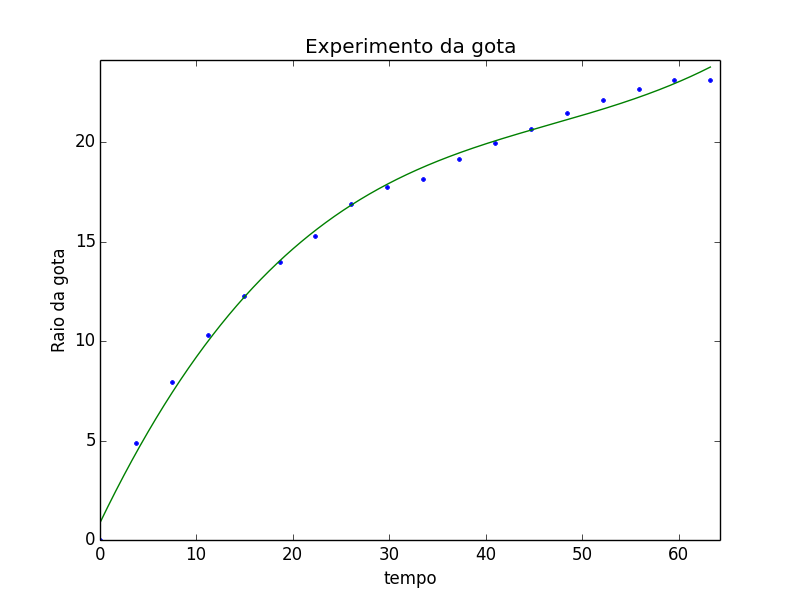
\includegraphics[width=12cm,height=9cm]{imgs/raio_gota.png}
\caption{ADD LEGENDA.}
\label{gota}
\end{figure}

\newpage
\section{Conclusões}
O passeio aleatório é um protótipo para vários modelos estocásticos os quais
as transições só podem ser feitas entre vizinhos. Ou seja, esse protótipo serviu para analizar o experimento da gota, embora esse experimento não seja um modelo físico muito preciso.

\end{document}




